\chapter{CPUスケジューリング}
プロセス(スレッド)の実行順序を決めることをスケジューリングと呼ぶ\footnote{
プロセスとスレッドの両方にあてはまることが多いので,
この章ではプロセスのスケジューリングを前提に議論する.}.
システム内で最も貴重な資源であるCPUの割当てを決める重要な機能である.

\section{評価基準}
スケジューリングの良し悪しを判断する評価基準には次のようなものがある.

\begin{itemize}
\item {\bf スループット(Throughput)} \\
単位時間あたりに処理できるジョブ数のことである.
大きい方が良い.

\item {\bf ターンアラウンド時間(Turnaround time)} \\
プロセスが実行できるようになってから終了するまでの時間のことである.
短いほうが良い.
バッチ処理で,
ユーザがジョブを提出してから実行結果の印刷物が届くまでの時間を
イメージすると分かりやすい.

\item {\bf レスポンス時間(Response time)} \\
対話的なシステム(TSSやデスクトップパソコン)において,
ユーザが操作した影響で出力が変化し始めるまでの時間である.
例えば,エンターキーを入力したあと画面が変化を始めるまでの時間である.
対話的なアプリケーションの操作性に大いに影響がある.
当然,短いほうが良い.

\item {\bf 締め切り(Deadline)} \\
制御用に用いられる{\bf リアルタイムシステム(Real-time system)}では,
決められた時刻(締め切り)までに結果を出すことが求められる.
必ず時間を守らなければならない場合を
{\bf ハードリアルタイム(Hard real time)},
できる限り時間を守らなければならない場合を
{\bf ソフトリアルタイム(Soft real time)}と呼ぶ.
オペレーティングシステムは,
制御用プロセスが締め切りを守ることができるスケジューリングを行う必要がある.

\item {\bf その他} \\
システムの使用方法などにより様々な評価基準が考えられる.
例えば,
モバイルデバイスではバッテリーために{\bf 省エネルギー}が評価基準になり得る.
\end{itemize}

\section{システムごとの目標}
システムの種類によって,
スケジューリングの目標は異なる.
\tabref{schedulingObjective}に概略をまとめる.

\begin{itemize}
\item {\bf メインフレーム} \\
バッチ処理を行う場合はユーザとの対話的な処理ではないので,
{\bf スループット}を優先する.
例えば,コンテキストスイッチにも処理時間が必要なので,
プリエンプションを行わないスケジューリング方式を採用し,
コンテキストスイッチの回数を少なくすること等が考えられる.
また,ユーザが結果を早く受取ることができるように,
{\bf ターンアラウンド時間}にも気を使う必要がある.

\item {\bf ネットワークサーバ} \\
ネットワークに接続され,
複数のクライアントから同時に多数の要求を受付けて処理する.
この場合は,
クライアントを操作しているユーザの操作性を損なわない{\bf レスポンス時間}と,
多数の要求を処理するための{\bf スループット}が両立することが望まれる.
両者のバランスが良いスケジューリングが求められる.

\item {\bf デスクトップパソコン} \\
一人のユーザが独占して使用するコンピュータである.
ユーザは,複数の処理を同時にすることは少ない.
ユーザの操作に素早く反応するために{\bf レスポンス時間}が重要である.
例えば,ユーザがワードプロセッサを操作している間に
バックグラウンドでメールの着信チェックを行うプロセスが動く場合,
ワードプロセッサが軽快に動くことを重視し,
メールの着信チェックプロセスの性能が落ちても構わない.
ユーザが直接操作するプロセスを優先するスケジューリングが求められる.

\item {\bf モバイルデバイス} \\
ノートパソコンやスマートフォンのようなシステムでは,
基本的にはデスクトップパソコンと同じように{\bf レスポンス時間}が重視される.
しかし,バッテリーで駆動される場合は
消費電力が少なくなるような工夫も必要である.
例えば,プロセスの切換え頻度を少なくすることで,
エネルギーの消費を小さくするスケジューリングを採用することが考えられる.

\item {\bf 組込み制御用のコンピュータ} \\
{\bf 締め切り}までに処理を完了することが重要である.
例えば,時速50kmで走行するエレベータ\footnote{
高層ビルのエレベータの中にはもっと高速なものもある.
}の制御コンピュータが,
1秒遅刻してブレーキを掛けたらどうなるだろうか.
時速50kmは秒速13mなので,エレベータは13m行き過ぎて停まることになる.
最上階,または,最下階を目指しているとき13m行き過ぎると
エレベータは天井か床に激突してしまう.
エレベータのブレーキ制御プロセスは{\bf ハードリアルタイム}に分類できる.
同じエレベータでも,
現在階数の表示はタイミングが少し遅れても大きな影響はない.
エレベータの階数表示プロセスは{\bf ソフトリアルタイム}に分類できる.
\end{itemize}

\begin{mytable}{btp}{スケジューリングの目標}{schedulingObjective}
  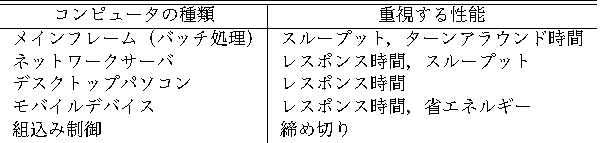
\includegraphics[scale=1.0]{Tbl/schedulingObjective.pdf}
\end{mytable}

\section{プロセスの振舞}
一般に,プロセスは計算と入出力を繰り返す.
計算と入出力にかかる時間の割合に応じて,
二種類のプロセスに分類できる.

\subsection{CPUバウンドプロセス}
例として,動画を圧縮するビデオエンコーディング・プロセスを考えてみよう.
プロセスは,\figref{cpuIoBound}(a)に示すように,次の三つの処理を繰り返す.

\begin{enumerate}
\item 未圧縮の動画ファイルを少し読む.
\item 圧縮処理を行う.
\item 結果を圧縮済み動画ファイル書込む.
\end{enumerate}

ビデオエンコーディング・プロセスはCPUが行う圧縮処理に長い時間がかかり,
入出力にかかる時間が短い.
このようにCPU処理にかかる時間が相対的に長いプロセスのことを
{\bf CPUバウンド(CPU-bound)プロセス}と呼ぶ.
また,CPUが使用される期間を{\bf CPUバースト(CPU burst)},
I/Oが使用される期間を{\bf I/Oバースト(I/O burst)}と呼ぶ.
CPUバウンドプロセスは長いCPUバーストと短いI/Oバーストを持つ.

\begin{myfig}{btp}{CPUバウンドとI/Oバウンドプロセス}{cpuIoBound}
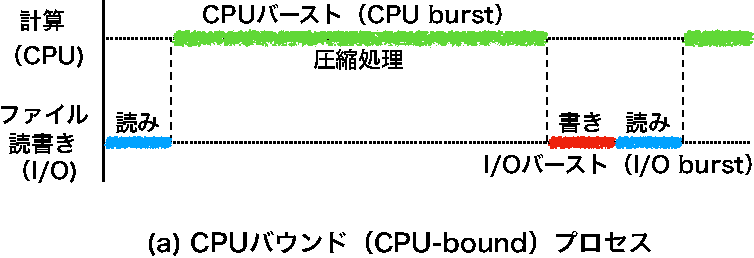
\includegraphics[scale=0.66]{Fig/cpuBound-crop.pdf}
\vspace{0.8cm}
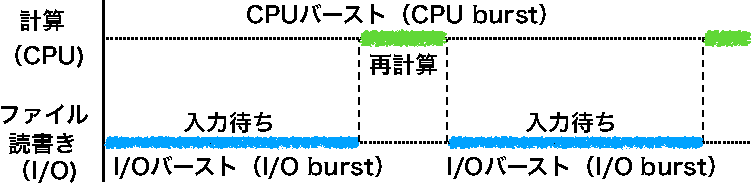
\includegraphics[scale=0.66]{Fig/ioBound-crop.pdf}
\end{myfig}

\subsection{I/Oバウンドプロセス}
二つ目の例としてスプレッドシート・プロセスを考えてみよう.
スプレッドシート・プロセスは,
まず,ユーザが何れかのセルにデータを入力するのを待つ.
次に,入力されたデータを用いてスプレッドシートの再計算を行い結果を表示する.
ユーザがセルにデータを入力するたびに同様な処理を繰り返す.
このプロセスは\figref{cpuIoBound}(b)に示すように,
ユーザ操作を待つ長い入力待ちと,
再計算と表示を行う短いCPU処理を行う.
このような,長いI/Oバーストと短いCPUバーストを持つプロセスを
{\bf I/Oバウンド(I/O-bound)プロセス}と呼ぶ.

\section{スケジューリング方式}
いくつかの代表的なスケジューリング方式を紹介する.

\subsection{First-Come, First-Served(FCFS)スケジューリング}
Ready状態になった順(到着順)に実行する方式である.
Running状態になったらブロックするまで実行を継続する.
プリエンプションはしない.
以下の例ではCPUバースト一回分の期間しか示さないが,
実際は,\figref{cpuIoBound}に示すようにCPUバースが繰り返し発生する.

FCFS方式は実行可能列をFIFOにするだけで実現できるが性能は良くない.
例えば次の三つのプロセスが時刻0で,
$P_1$,$P_2$,$P_3$の順にReady状態になったとする.

\begin{center}
\begin{tabular}{c c c}
プロセス & 到着時刻 & CPUバースト時間(ms) \\
\hline
$P_1$    & 0 & 100 \\
$P_2$    & 0 & 20 \\
$P_3$    & 0 & 10 \\
\end{tabular}
\end{center}

この時,三つのプロセスの実行開始・終了の時刻を図で表すと次のようになる.

\begin{center}
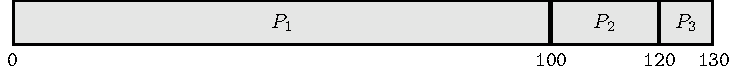
\includegraphics[scale=1.0]{GanntChart/fcfs1.pdf}
\end{center}

平均ターンアラウンド時間を計算すると,
$(100+120+130) / 3 = 117$ ms となる.
もしも,プロセスの到着順が$P_2$,$P_3$,$P_1$の順だったとすると,
三つのプロセスの実行開始・終了の時刻は図のようになる.

\begin{center}
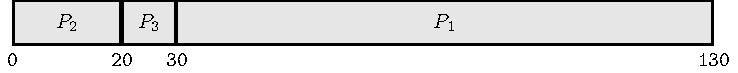
\includegraphics[scale=1.0]{GanntChart/fcfs2.pdf}
\end{center}

この場合の
平均ターンアラウンド時間を計算すると,
$(20+30+130) / 3 = 60$ ms となる.
このように,FCFSでは最悪な平均ターンアラウンド時間を選択することもある.
プリエンプションをしないので,
一旦,CPUバウンドなプロセスが実行を開始すると,
他のプロセスは長い時間待たされる.

\subsection{Shortest-Job-First(SJF)スケジューリング}
SJF方式\footnote{皆さんの教科書ではSPTのこと.}は,
平均ターンアラウンド時間を最小にするスケジューリング方式である.
SJF方式ではCPUバースト時間が短いものを先に実行するようにスケジューリングする.
実行可能列はCPUバースト時間が短い順にソートされている.

三つのプロセスがあった時,
実行順に各プロセスの実行時間が$T_1$,$T_2$,$T_3$とすると,
平均ターンアラウンド時間は,
$(T_1+(T_1+T_2)+(T_1+T_2+T_3))/3=T_1+T_2*2/3+T_1/3$となるり,
先に実行したプロセスの実行時間ほど結果に及ぼす影響が大きいことが分かる.
実行時間が短いプロセスを先に実行するスケジューリング方式は,
平均ターンアラウンド時間を最小にする.

前出の三つのプロセスをSJF方式でスケジューリングした時の,
実行開始・終了時刻は次の図のようになる.

\begin{center}
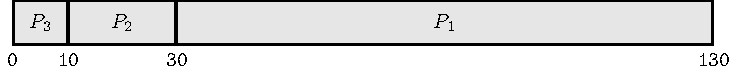
\includegraphics[scale=1.0]{GanntChart/sjf1.pdf}
\end{center}

この図より平均ターンアラウンド時間を求めると
$(10+30+130)/3 = 57$ ms となり,これまでで最短である.
しかし,次回のCPUバースト時間を知ることは一般には不可能なので,
SJF方式は現実的な方式ではない.
次回のCPUバースト時間を予測することで擬似的なSJF方式を実現する.

次回のCPUバースト時間を予測する方法として,
指数平滑平均(exponential average)を用いる例を紹介する.
次回の予測時間を$T_{n+1}$,
前回の予測時間を$T_{n}$,
前回の実際のCPUバースト時間を$t_{n}$とすると,
$0 \le \alpha \le 1$の時,
指数平滑平均は次の式で表すことができる.

\[T_{n+1} = \alpha t_n + ( 1 - \alpha ) T_n\]

この式から

\[T_{n+1} = \alpha t_n + ( 1 - \alpha ) \alpha t_{n-1} + \dots +
 ( 1 - \alpha )^j \alpha t_{n-j} + \dots + (1 - \alpha )^{n+1} T_0 \]

を得る.$\alpha = 0.5$ の場合は,

\[T_{n+1} = 0.5 t_n + 0.5^2 t_{n-1} + \dots +
0.5^{j+1} t_{n-j} + \dots + 0.5^{n+1} T_0 \]

となる.
この式は,過去のCPUバースト時間を,
最近のものほど大きな重みを付けて平均したものになっている.
つまり,次回のCPUバースト時間は,
過去のCPUバースト時間と同程度であろうとの仮定に基づいた予測値を計算している.

\subsection{Shortest-Remaining-Time-First(SRTF)スケジューリング}
SRTF方式\footnote{皆さんの教科書ではSRPTのこと.}は,
プリエンプション付きのSJF方式である.
プロセスがReady状態になるとき,
このプロセスのCPUバースト時間と
実行中のプロセスの{\bf 残りCPUバースト時間}とを比較し,
{\bf 残りCPUバースト時間}の方が長いときプリエンプションをおこす.
次の例でSJTとSRFTを比較してみよう.

\begin{center}
\begin{tabular}{c c c}
プロセス & 到着時刻 & CPUバースト時間(ms) \\
\hline
$P_1$    & 0  & 60 \\
$P_2$    & 10 & 40 \\
$P_3$    & 60 & 30 \\
\end{tabular}
\end{center}

三つのプロセスをSJFでスケジューリングした場合は次の図のようになる.

\begin{center}
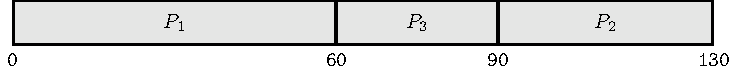
\includegraphics[scale=1.0]{GanntChart/sjf2.pdf}
\end{center}

平均ターンアラウンド時間を計算すると,
$((60-0)+(90-10)+(130-60))/3=70$ ms となる.
三つのプロセスをSRTFでスケジューリングした場合は次の図のようになる.

\begin{center}
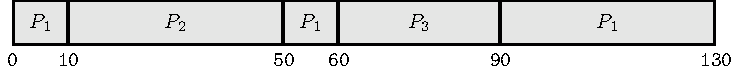
\includegraphics[scale=1.0]{GanntChart/srtf1.pdf}
\end{center}

$P_2$が到着した時,
$P_2$のCPUバースト時間($40$ ms)の方が
$P_1$の残りCPUバースト時間($60 - 10 = 50$ ms)より短いので,
$P_1$はプリエンプションし$P_2$が先に実行される.
$P_3$が到着した時も同様である.
平均ターンアラウンド時間を計算すると,
$((130-0)+(50-10)+(90-60))/3=67$ ms となり,
SJFよりも改善されている.

\subsection{Round-Robin(RR)スケジューリング}
{\bf タイムシェアリングシステム(TSS)}で使用された方式である.
{\bf クォンタム時間(time quantum)},または,
{\bf タイムスライス(time slice)}と呼ばれる10 ms 〜 100 ms 程度の
一定の時間が予め決められている.
実行可能列はFIFOになっている.
実行可能列の先頭のプロセスにCPUが割り付けられてRunning状態になる.
プロセスの実行が{\bf クォンタム時間}連続するとプリエンプションが発生し,
プロセスは実行可能列の最後尾に付け加えられる.

{\bf クォンタム時間($q$)}が短いと{\bf レスポンス時間}が短くなり,
対話的な処理が円滑に行える.
例えば,10個のプロセスがCPUを奪い合うような状況でも,
$q = 10$ ms なら$100$ ms に一度は全てのプロセスにCPUが割り付けられる.
しかし,$q$ を小さくしすぎるとコンテキストスイッチの回数が多くなり,
オーバーヘッドが大きくなる.
逆に $q$ が長いとFCFSと同じ結果になる.

前出の三つのプロセスをRR方式($q = 10$ ms)でスケジューリングした例を
次の図に示す.
なお,
新規プロセスと,
クォンタム時間を使い切りプリエンプションしたプロセスが,
同時に実行可能列に追加される場合は,
新規プロセスを優先することにする.

\begin{center}
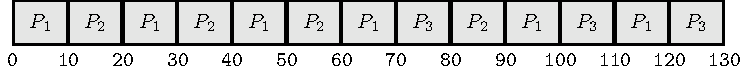
\includegraphics[scale=1.0]{GanntChart/rr1.pdf}
\end{center}

平均ターンアラウンド時間を計算すると,
$((120-0)+(90-10)+(130-60))/3=90$ ms となる.
次に $q = 50$ ms でスケジューリングした例を示す.

\begin{center}
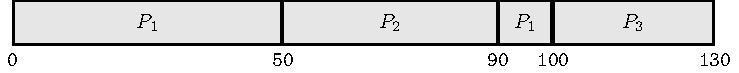
\includegraphics[scale=1.0]{GanntChart/rr2.pdf}
\end{center}

平均ターンアラウンド時間を計算すると,
$((100-0)+(90-10)+(130-60))/3=83$ ms となる.
$q = 50$ ms でスケジューリングした方が,
平均ターンアラウンド時間が短くなった上に,
コンテキストスイッチの回数が少ない.
このようなプロセスの集合に対しては,
$q = 10$ ms はクォンタム時間が短すぎると言える.

\subsection{Priority (優先度順)スケジューリング}
プロセス毎に決められた{\bf 優先度}を基に行うスケジューリング方式である.
実行中に優先度が変化する{\bf 動的優先度}を用いる方法と,
プロセス生成時に決められ変化しない{\bf 静的優先度}を用いる方法がある.
TacOSは{\bf 静的優先度}を用いる優先度順スケジューリング方式を用いる.
SRTF方式は,
次回CPUバースト時間が短い順の{\bf 動的優先度}方式と考えられる.

優先度順スケジューリング方式の問題点は,
優先度の低いプロセスが全く実行されない{\bf スタベーション(stavation)}が
発生することである.
これの対策として,
実行可能列に留まるプロセスの優先度を徐々に高くしていく
{\bf エージング(aging)}が用いられる.
実行可能列に長く留まるプロセスは優先度が高くなり,
やがて実行される.

\subsection{Multilevel Feedback Queue(FB)スケジューリング}
Windows,macOS,UNIX等で広く使用されているスケジューリング方式である.
\figref{multilevelFeedbackQueue}に示すように実行可能列を優先度別に複数設ける.
優先度が近いプロセスが同じ実行可能列に登録される.
同じ実行可能列ではRR方式でスケジューリングするので\footnote{
実行可能列ごとに,異なるスケジューリング方式を採用することも可能である.
},
列内でプロセスの順番は優先度とは関係がない.
CPUを割り付ける際は,
優先度の高い実行可能列から順に調べ,
最初に見つかった空ではない実行可能列を使用する.

\myfigure{btp}{scale=0.6}{Fig/multilevelFeedbackQueue-crop.pdf}
{Multilevel Feedback Queue}{multilevelFeedbackQueue}

プロセスの優先度は動的に変化する方式を用いる.
CPUバウンドなプロセスの優先度は急激に引き下げられ,
プロセスは下位の実行可能列に移動する.
長く実行可能列に留まっているプロセスは,
{\bf エージング}により優先度を引き上げられ上位の実行可能列に移動する.
実行中のプロセスより上位の実行可能列にプロセスが登録されると
プリエンプションが発生し,プロセスが切り換わる.
これにより{\bf スタベーション}を避ける.

\section{TacOSのスケジューラ}
実行可能になったプロセスをスケジューリングするプログラムを{\bf スケジューラ}と呼ぶ.
スケジューラの例として,
TacOSのスケジューラのソースプログラムを\figref{tacosSch}に示す\footnote{
%\figref{tacosSch}はTacOSのソースコード
\url{https://github.com/tctsigemura/TacOS/blob/master/os/kernel/kernel.cmm}
の一部である.}.
TacOSの実行可能列は,
PCBの番兵付き重連結環状リストとして表現する
(\figref{tacosReadyQueue}参照).

\begin{figure}[btp]
\lstinputlisting{Lst/sch.cmm}
\caption{TacOSのスケジューラ・ソースプログラム}
\label{fig:tacosSch}
\end{figure}

\begin{quote}
\begin{description}
\item[1〜7行] 関数\|insProc()|は,
実行可能列にPCBを登録するために使用される.
スケジューラ以外からも呼出される汎用的なものである.

\item[9〜19行] 関数\|schProc()|がスケジューラである.
\|enice|がプロセスの優先度である.
\|enice|は値が小さい方が優先度が高い.
スケジューラは,
実行可能列(\|readyQueue|)を番兵PCBの次のPCBから開始して(14行),
挿入するプロセスの\|enice|より大きいものを探す(15,16行).
大きいものを見つけたら\|insProc()|を使用して,
見つけたPCBの直前に新しいプロセスのPCBを挿入する(17行).
実行可能列の最後には,常時IdleプロセスのPCBが置かれている
(\figref{tacosReadyQueue}参照).
Idleの\|enice|は最大値に設定されているので15行のループは必ず正常に終了する.

現在の実装では,\|enice|はプロセス生成時に\|nice|と同じ値に設定され,
その後は変化しない.
TacOSは{\bf 静的優先度}を用いる{\bf 優先度順スケジューリング方式}を用いていることになる.
将来,\|enice|の値を動的に変化させるように変更すれば,
{\bf 動的優先度}方式になる.

\|setPri()|関数はPSWの割込み許可フラグを操作するために使用している.
詳しくは「\ref{setPri} setPri()関数」で説明する.
\end{description}
\end{quote}
